% Paper B manuscript for Sociological Methods & Research (anonymized for double-anonymized review).
% Author names, affiliations and acknowledgements live in title_page.tex (separate upload).
% Claim source: planning/TWO_PAPER_CLAIM_LOCK.md, Amendments C7 (2026-10-18) to C9.1 (2026-10-20), with
% planning/sprint_2026-10-11/paper-b-tier1/NUMBERS_TABLE.csv (sha256 71ee7c8c...86a4, 562 rows). The
% descriptive follow-up analyses (surface D) use the C9 rows; the C9-4 rows still owe a cross-family audit.
% TODO(Augusto): swap to the SMR Overleaf template at submission; this preamble follows the SMR
% format rules (12 pt, double spacing, 1.25 in margins, footnotes, author-date references).
\documentclass[12pt]{article}
\usepackage[T1]{fontenc}
\usepackage[utf8]{inputenc}
\usepackage[margin=1.25in]{geometry}
\usepackage{lmodern,microtype,amsmath,amssymb,booktabs,tabularx,array,graphicx,xcolor}
\usepackage{tikz}
\usetikzlibrary{positioning,arrows.meta}
\usepackage{setspace}
\usepackage[authoryear,round]{natbib}
\usepackage{xurl}
\usepackage[hidelinks]{hyperref}
\usepackage[labelfont=bf]{caption}
\setlength{\emergencystretch}{2em}
\widowpenalty=10000
\clubpenalty=10000
% Shared macros for the Paper B manuscript.
%
% \cl{<printed>}{<claim_id>[:field]} prints <printed>. The second argument names the row of
% planning/sprint_2026-10-11/paper-b-tier1/NUMBERS_TABLE.csv that the printed number comes from
% (fields: v value, lo ci_low, hi ci_high, n, pct = 100 x value, abs = |value|). A rebuilt table is a
% mechanical swap; tools/audit_numbers.py checks every \cl against the table at the printed precision.
% \dc{<printed>}{<key>} prints a design constant; the key resolves to the document that fixes it
% (allowlist in tools/audit_numbers.py).
\newcommand{\cl}[2]{\ensuremath{#1}}
\newcommand{\clh}[2]{\texttt{#1}}
\newcommand{\dc}[2]{#1}
\newcommand{\ci}[3]{[\cl{#1}{#3:lo}, \cl{#2}{#3:hi}]}
\newcommand{\GPS}{GPS}
\newcommand{\WVS}{WVS}
\newcommand{\DPO}{DPO}
\newcommand{\Aprim}{\ensuremath{A}}


\title{Synthetic Cultural Agents as Measurement Instruments: A Preregistered Evaluation from Cross-National Anchor to Survey Respondents}
\author{}
\date{}

\begin{document}
\maketitle
\thispagestyle{empty}
\begin{abstract}
\noindent Synthetic respondents built from large language models promise a cheap first reading of survey items before fielding, yet their value as a screening instrument is rarely tested on items they were not built for. We evaluate synthetic cultural agents, which compile the signs of declared country-level preference benchmarks into parameter adapters through a regularized pairwise choice model, as a scoring instrument for new item text. Under a preregistered protocol, the adapters alone assigned a dimension and a direction to candidate World Values Survey items before any human value was read. Against the existing survey, the selected items predict the direction of cross-national differences better than random assignment, but the signal is weak and no preference dimension passes both a second-bank check and the held-out screen. A factorial over sign profiles shows that the dimensions are entangled, more so under prompting. Because the human criterion is retrospective, pre-piloting remains a prospective use that this paper does not test.
\end{abstract}

\noindent\textbf{Keywords:} synthetic respondents; large language models; survey item screening; preregistration; cross-national measurement; direct preference optimization.

\clearpage
\doublespacing
\section{Introduction}\label{sec:introduction}

Cross-national survey programs fix their items long before they see how those items behave. A question on trust in institutions or on willingness to take risks must be translated, pretested and fielded in many countries before a researcher learns whether its country-level differences follow the construct it was meant to capture. Language models offer a cheap first reading of such items \citep{argyle2023,horton2023,buskirk2026}, but whether a model deserves that role is a question about a chain of links and not about a single accuracy figure. We evaluate one instrument along the chain from an anchor, a declared country-level benchmark, through the instrument, a set of adapters trained on the signs of that benchmark, to respondents, the people whose survey answers the instrument is meant to inform. We report where along the chain the instrument holds and where it fails.

That role has drawn a literature that is mostly cautionary. Synthetic responses are sensitive to prompt wording, compress the variance of human answers, and can misportray and flatten identity groups \citep{bisbee2024,boelaert2025,wang2025}, and they depend on the order and labelling of answer options \citep{dominguezolmedo2024}. The alignment procedures that make models usable change how faithfully they simulate population attitudes \citep{lyman2025}. Methodological work in this journal concludes that validation against human data remains essential, and proposes designs that treat model output as potentially informative observations beside a human gold standard \citep{kozlowski2025,broska2025}. Most of the empirical work asks whether a model reproduces answers that people already gave, whether the model is prompted \citep{santurkar2023,durmus2024} or fine-tuned on survey response distributions \citep{cao2025,suh2025}. In the fine-tuned case the human survey sits inside the training signal. Language-model pretesting, for its part, has been studied as flaw detection in question wording \citep{sturgis2026}. Whether an instrument can say which new items will separate countries in an intended direction is a different test, and it needs a decision rule fixed before the human criterion is read.

The three links of the chain are as follows. The anchor is the Global Preferences Survey \citep[GPS;][]{falk2018}, whose country-level scores on six preference dimensions supply the signs that define what the instrument is meant to carry. The instrument is a set of parameter adapters trained on synthetic response pairs that those signs label. The respondents are the people who answered Wave~7 of the World Values Survey (WVS). A favorable result at one link does not carry to the next. This is the measurement lens that has been proposed for the evaluation of generative systems in general \citep{wallach2025}, and we apply it to one instrument under a preregistered protocol. Prompted models have already been compared with the GPS across countries and found to be weak proxies for it \citep{chen2026}. We ask the question of an instrument trained on the signs of that benchmark.

The instrument, which we call synthetic cultural agents, is built from signs alone. Each country's sign profile on the six GPS dimensions deterministically labels a shared bank of paired synthetic responses, and Direct Preference Optimization \citep{rafailov2023}, read as a regularized Bradley--Terry pairwise choice model, fits one adapter per profile. The adapters are scored on survey items with prompts that never name a country. What is specific to the construction is its training signal, which consists of six declared signs and no human answers, together with the unnamed group at evaluation. The construction is inspectable: the researcher controls which aggregate moments enter, the sign rule that turns them into labels, and whether the group is named. We built it in the development stage of this study, on a purposive panel of \dc{16}{dev_countries} countries, and evaluate it here on every country covered by both the GPS and the WVS Wave~7, with a second set of adapters for all \dc{64}{cells} possible sign profiles on a newly generated scenario bank.

The evaluation has four parts. The first asks whether training installs the synthetic labels on pairs the adapters never saw, whether the adapters' order of countries on the anchor survives a change of scenario bank, and whether a prompt that names the country or one that states the signs does as well. The second is a preregistered screen of \dc{223}{pool_items} WVS Wave~7 items that no adapter was built for. A probe that reads only the adapters' scores assigns each item a dimension and a direction, a fixed rule selects the items with the strongest assignments, and only then are the selected items compared with the human country differences. That criterion is retrospective, because the survey existed before the probe, and we say so wherever the screen is reported. The third part is a factorial over the \dc{64}{cells} sign profiles, which asks whether the six declared dimensions behave as separate inputs. The fourth consists of descriptive follow-up analyses that set the adapters beside the respondents' composite scores and answer distributions. The second-bank check, the screen and the factorial follow the preregistration. The follow-up analyses were added after the registered results had been read, and they earn no claim.

At the first link the instrument holds in a limited sense. Training installs the synthetic labels on scenarios the adapters never saw. On trust the adapters keep the GPS order of countries when the scenario bank is replaced, and a prompt that names the country does not. A prompt that states the same six signs keeps the trust order as well, and the registered contrast between adapters and that prompt is unresolved. The trust order therefore belongs to the declared signs, and the evidence cannot credit the trained weights over a prompt.

The remaining links are weaker. Each declared sign moves its own surface in the intended direction and also moves the surfaces of other dimensions, often by more, so the dimensions are entangled; a behavioral decomposition shows trust spared where the other five signs add little to its surface, and shows them carrying most of the variation on the others. Entanglement across cultural dimensions has been reported for activation steering \citep{dangmasud2026}, and the factorial here measures it for trained adapters and for a prompt. The retrospective screen of held-out items gives a weak signal: the registered null is rejected, yet the bootstrap interval reaches zero, and the registered contrasts do not distinguish the adapters from careful readers of the questionnaire on the few items they share. No dimension passes both the second-bank check and the screen. Descriptively, the adapters' order of countries does not detectably agree with the respondents' composite on any surface, and the agreement between the GPS and those respondents is itself loose on these items.

Two questions that a single agreement figure would merge separate here. One asks whether the instrument keeps the anchor's order of countries. The other asks whether it reproduces the answer distributions of respondents. On the first, the adapters keep the order on trust and a country-named prompt does not. On the second, the adapters sit farther from the survey's answer distributions than the base model does, and the country-named prompt sits closer. We report this as a descriptive contrast between two questions. The separation of group-level order from distributional fidelity is known \citep{dasilva2026}, and a country name has been found to recover a country ranking on other items in the European Social Survey \citep{wangc2026}. The crossing reported here concerns one anchor, one instrument family and the trust order of one benchmark. It was not preregistered, and it does not show that any arm matches respondents.

Our contributions are three.
\begin{enumerate}
\item \textbf{A chain-wise evaluation of one instrument.} We place the instrument between a declared anchor and a human survey and report, link by link, what a favorable or an unfavorable result permits, including the contrast between keeping the anchor's order of countries and approaching respondents' answer distributions.
\item \textbf{A preregistered retrospective screening protocol.} We specify, register and run a screen of new survey items with a probe fixed before any human value was read, a permutation null that absorbs the probe's own selection rate, a human ceiling from two survey waves, and two comparators that read only the questionnaire.
\item \textbf{A factorial over sign profiles.} We vary all six declared signs jointly to measure how far each dimension moves the surfaces of the others in trained adapters and under a prompt that states the same signs, and we add a descriptive decomposition of where trust is spared.
\end{enumerate}

What the paper shows is bounded by its design. For one anchor, one instrument family and one base model, it shows that the declared signs carry the trust order, that the instrument keeps the direction of each sign and not the separation of dimensions, that a preregistered screen finds a weak retrospective signal, and that keeping an anchor's order of countries and approaching respondents' answer distributions are different questions with different answers. It does not show that trained weights improve on a prompt that states the same signs. It does not show agreement with respondents beyond the weak retrospective signal. It does not show that screening would change which items a researcher fields, because the WVS Wave~7 file existed before the probe, the item pool and the adapters, and pre-piloting is a prospective use that remains untested. The instrument is built from signs alone, so it carries no information about magnitudes or about variation among people within a country, and its readings concern differences among countries. Within these bounds it is an inspectable instrument that a survey designer can consult beside human pretesting. It is a complement to pretesting and fielding, and the evidence gives no reason to use it in their place. Section~\ref{sec:background} places the instrument among current uses of synthetic respondents and in the measurement literature on cross-national comparability. Section~\ref{sec:instrument} describes the construction, Section~\ref{sec:design} the evaluation design and its registration, Section~\ref{sec:results} the results, and Section~\ref{sec:discussion} what they permit a researcher to do.

\section{Synthetic Respondents as Measurement Instruments}\label{sec:background}

\paragraph{Synthetic respondents and the criterion they need.} A language model conditioned on a description of a population can be asked to stand in for a sample of its members. In silicon sampling the description enters the prompt and the model's answer distribution is read as an estimate of the population's \citep{argyle2023}; in the homo silicus program the model plays an economic agent in a stylized decision problem \citep{horton2023}; a systematic review maps how fast these uses have spread across survey research \citep{buskirk2026}. The evidence on prompted models is summarized in the introduction. Fine-tuning on survey responses is one response to it \citep{suh2025,cao2025,krsteski2026}. Two reviews in this journal draw the methodological conclusion that matters here. \citet{kozlowski2025} conclude that validation against human data remains essential, and \citet{broska2025} propose a design in which model predictions are potentially informative observations and human subjects remain the gold standard. Both require a criterion against which the synthetic reading can fail. Our evaluation supplies one criterion for each link of the chain.

\paragraph{Construct, measure, and anchor.} Three objects have to be kept apart. A construct is a theoretical preference attribute, such as generalized trust. A measure operationalizes it through observed answers, such as the response distribution to a WVS question about whether most people can be trusted. An anchor is an aggregate score that conditions the instrument, such as a country's GPS trust coordinate. The GPS supplies anchors for six economic preferences (trust, risk taking, patience, altruism, positive reciprocity and negative reciprocity), measured with experimentally validated modules in a common design across countries \citep{falk2018}. We treat these coordinates as declared aggregate moments: the researcher chooses them, and nothing in the construction certifies them as the right moments for a given survey. Mapping a WVS item to a GPS dimension makes the item a candidate indicator, and an average of such items is a proposed composite until its interpretation is supported. Agreement between instrument and anchor, between instrument and people, and between anchor and people across countries are therefore three different facts, and they are the three comparisons that the chain makes. The multitrait--multimethod logic of \citet{campbellfiske1959} applies directly: the human survey is the other method, and an instrument that agrees with its own anchor has passed a construction check without yet meeting a criterion.

\paragraph{Cross-national comparability.} The unit of analysis is the country. Country-level agreement does not establish that an item measures the same construct for individuals in different countries. Loadings and intercepts can differ across groups in ways that leave country means comparable for some purposes and misleading for others \citep{steenkamp1998,davidov2014}. Work in this journal argues that composite scores aggregated to the country level can suffice for simple group comparisons despite noninvariance, while understating uncertainty \citep{bratt2025}, and that unaddressed measurement error and, less so, noninvariance bias multilevel estimates \citep{pokropek2025}. We adopt the same posture. Every comparison with respondents below is a group-level directional question about country rankings, with no claim about invariance or individual-level validity.

\paragraph{The empty cell.} Prior evaluations score models on questions whose human answers are known, usually with the population named in the prompt, and fine-tuning approaches learn from human survey responses. The question here is, link by link, what an instrument built from declared aggregate inputs alone preserves of its anchor and of the respondents' answers, with the selection rule and inference for new items registered before the human criterion is read and with comparators that read only the questionnaire. Section~\ref{sec:design} describes such an evaluation and Section~\ref{sec:results} reports it.

\section{The Instrument}\label{sec:instrument}

The instrument maps declared aggregate preference signs into choice policies and reads those policies on survey items without naming any country. We describe the construction, the two cohorts of adapters it produced, and the two prompt routes they are compared with. Throughout, a language model is treated as a conditional distribution over response sequences given a prompt \citep{ludwig2026}.

\subsection{From declared signs to a shared pair bank}

Let $z_c=(z_{c1},\ldots,z_{cK})$ be the GPS coordinates of country $c$ on the $K$ dimensions trust, risk taking, patience, altruism, positive reciprocity and negative reciprocity. Only the sign profile $s_c$, with $s_{ck}=1\{z_{ck}\geq 0\}$, enters the construction. A teacher model and a response generator produce a shared bank of scenarios, each with two responses intended to express a higher and a lower level of one dimension $k_i$. For country $c$, the chosen and rejected responses on pair $i$ are
\begin{equation}
(y_{w,ci},\,y_{\ell,ci})=\begin{cases}(y_i^{+},\,y_i^{-}), & s_{c,k_i}=1,\\ (y_i^{-},\,y_i^{+}), & s_{c,k_i}=0.\end{cases}
\label{eq:sign_rule}
\end{equation}
The scenario and response text is identical for every country; only the label changes. No scenario names a country and none reuses WVS question wording, and the intended loading of each pair is a generator judgment rather than a verified trait manipulation. Two countries with the same sign profile receive identical labels, so the instrument cannot distinguish them, and nothing in the construction carries the magnitude $|z_{ck}|$.

\subsection{Preference optimization as regularized pairwise choice}

Each sign profile is fitted with Direct Preference Optimization. Under the Bradley--Terry model, the probability that $y_w$ is chosen over $y_\ell$ after prompt $x$ is $\sigma\{r(x,y_w)-r(x,y_\ell)\}$, with $\sigma$ the logistic function and $r$ a latent utility index. DPO writes the index as $r(x,y)=\beta\log\{\pi_\theta(y\mid x)/\pi_{\mathrm{ref}}(y\mid x)\}$ up to a prompt-specific constant that cancels from pairwise differences, and minimizes the negative log likelihood of the labeled pairs,
\begin{equation}
\mathcal{L}_c(\theta)=-\frac{1}{|\mathcal{D}_c|}\sum_{(x,y_w,y_\ell)\in\mathcal{D}_c}\log\sigma\!\left\{\beta\log\frac{\pi_\theta(y_w\mid x)}{\pi_{\mathrm{ref}}(y_w\mid x)}-\beta\log\frac{\pi_\theta(y_\ell\mid x)}{\pi_{\mathrm{ref}}(y_\ell\mid x)}\right\}.
\label{eq:dpo}
\end{equation}
The parameter $\beta$ penalizes departures from the reference policy, which makes the estimator a regularized Bradley--Terry fit \citep{bradleyterry1952,rafailov2023}. Because the labels are deterministic, the likelihood serves as a fitting criterion and says nothing about the noise in human choices. Each adapter is a low-rank update to a quantized Llama~3.1 8B Instruct base model \citep{hu2022,dettmers2023}, trained jointly on all six dimensions for one epoch on \dc{526}{train_rows} of the \dc{658}{bank_pairs} pairs, with LoRA rank \dc{16}{lora_r} and $\beta=\dc{0.1}{dpo_beta}$. A joint adapter does not isolate any single dimension; whether the dimensions separate in practice is the subject of the factorial diagnostic in Section~\ref{sec:design}.

\subsection{Two cohorts and two prompt routes}

The paper uses two sets of adapters. The first cohort has one adapter for each of the \dc{42}{countries} countries in the intersection of the GPS and WVS Wave~7, trained on the original scenario bank. These \dc{42}{countries} countries realize \dc{26}{profiles_realized} distinct sign profiles. The second cohort is trained on a second, independently generated bank of \dc{658}{bank_pairs} pairs under the same sign rule and the same text restrictions, and it contains one adapter for every one of the \dc{64}{cells} possible sign profiles of the six dimensions. Because the labels depend on the country only through its sign profile, each of the \dc{42}{countries} countries takes the adapter of its profile when country-level comparisons are needed; we verified that each country's labels on the second bank equal those of its profile. The \dc{64}{cells} profiles form a full $2^6$ factorial in the six sign bits. Each profile is a constructed design cell, and most of them are realized by no country.

The sign-profile prompt route gives the base model the same six signs in words, with no country name and no adapter. It carries the same declared information through a different channel, which makes it the natural comparison for the trained route. The country-named persona route replaces the neutral opening of the evaluation prompt with ``Answer this questionnaire as a typical adult living in'' followed by the country's name, and supplies no signs. It changes the information as well as the channel, because the model can draw on whatever it associates with the country name, which the sign rule never sees. Naming the population is the comparison a survey researcher would reach for first, so we score this route on all \dc{42}{countries} countries.

\subsection{Readout}

For an item $q$ with candidate response codes $j$, the instrument computes the teacher-forced log probability of each code after the rendered item prompt and normalizes over the supplied codes,
\begin{equation}
\widehat P_u(j\mid q)=\frac{\exp \ell_{uqj}}{\sum_h \exp \ell_{uqh}},
\qquad
y_{uq}=\sum_j g_q(j)\,\widehat P_u(j\mid q),
\label{eq:readout}
\end{equation}
where $\ell_{uqj}$ is the summed token log probability of code $j$ for unit $u$ (an adapter or a prompted profile) and $g_q$ is the item's recode. The score $y_{uq}$ is the expected recoded response. Apart from the persona route, no evaluation prompt names a country. The prompt template, the option order, the leading space before each code and the recode are frozen in a scoring specification whose hash every scoring run must reproduce before a model is loaded. On the original \dc{23}{strict_items}-item WVS battery, item scores are averaged into seven surfaces: trust, risk taking, altruism, positive reciprocity, negative reciprocity, and two separate patience items. We call this the strict battery. The normalized code probabilities are a scoring convention, and their dispersion need not match the response distributions of any human population.

\section{Evaluation Design}\label{sec:design}

The evaluation follows the chain, and each comparison permits one kind of statement. A construction check asks whether the adapters encode what they were trained on (anchor to instrument). A second-bank check asks whether the encoding of the anchor's order survives a change of scenario text. A factorial asks whether the declared dimensions behave as separate inputs. A held-out screen asks whether the instrument's readings of new items agree with an existing human survey (instrument to respondents). Descriptive follow-up analyses, added after the registered results had been read, place the instrument beside the respondents and beside its own training labels. Every number carries the label of the surface it was computed on (Table~\ref{tab:surfaces}), and numbers from different surfaces are never pooled.

\begin{table}[htbp]
\centering
\caption{Evaluation surfaces. Every number in the paper carries one of these labels.}\label{tab:surfaces}
\small
\renewcommand{\arraystretch}{1.15}
\begin{tabularx}{\textwidth}{@{}l>{\raggedright\arraybackslash}X>{\raggedright\arraybackslash}X>{\raggedright\arraybackslash}p{0.27\textwidth}@{}}
\toprule
Label & Units and items & Comparison & What it can show \\
\midrule
S1 & First-cohort country adapters (original bank), strict battery & Adapter--GPS rank correlation over countries; model side only & Whether a surface encodes its declared sign \\
S2 & Second-cohort profile adapters (second bank), each country mapped to its profile, strict battery & Same statistic and bootstrap as S1 & Whether that encoding survives a new scenario bank \\
H & Second-cohort adapters on held-out WVS Wave~7 items & Signed agreement of selected items with human country means, against GPS & Retrospective screen of new items against an existing survey \\
F & Second-cohort adapters and prompted profiles, strict battery & Main effects of the six sign bits on seven surfaces; model side only & Whether the declared dimensions separate \\
R & One profile retrained without a fixed seed & Score differences against the original adapter; model side only & Retraining noise for one unit \\
N & Two near-zero refits and size-matched controls & Composite shifts in profile standard deviations; model side only & Sensitivity of the sign rule's margin \\
P & Country-named persona prompt on the base model, strict battery & Persona--GPS rank correlation; paired difference with S1; model side only & Whether naming the country carries the GPS ordering \\
D & First-cohort adapters, second-cohort factorial and the persona routes, strict battery; descriptive follow-up analyses, not preregistered & Agreement with the GPS and with the WVS Wave~7 composite; distance to survey answer distributions; decomposition of main effects; held-out label recovery & A description of how the instrument relates to respondents and to its own labels; no test \\
\bottomrule
\end{tabularx}
\end{table}

\subsection{Second-bank check}\label{sec:design-bank}

For each surface of the strict battery, we compute the Spearman correlation between the adapters' surface composites and the GPS coordinate of the surface's own dimension over the \dc{42}{countries} countries, first for the first cohort (S1) and then for the second cohort with each country assigned its profile's adapter (S2). Intervals come from a profile-block bootstrap that resamples the \dc{26}{profiles_realized} realized sign profiles, with \dc{2,000}{boot_draws} draws, seed \dc{20261011}{seed_c3}, and percentile limits. The imprint set is the \dc{4}{imprint_dims} dimensions whose first-cohort interval excluded zero: trust, risk taking, positive reciprocity and altruism. Patience and negative reciprocity were flat in the first cohort and are reported without interpretation. The rule was fixed before the second cohort was trained: an imprint dimension whose second-bank interval includes zero is named, and no sentence about that dimension carrying over to the second bank is written. We also report the Pearson agreement between the two banks over the \dc{26}{profiles_realized} shared profiles, with a \dc{2,000}{boot_draws}-draw bootstrap over profiles. It measures how much the scenario text changes the instrument and involves no human data.

\subsection{The country-named prompt}\label{sec:design-persona}

The persona route (Section~\ref{sec:instrument}) was scored on the strict battery for each of the \dc{42}{countries} countries in one run on the frozen stack, after a rescoring of the base model that reproduced the banked base scores exactly. We compute the persona--GPS correlation for each surface (surface P) and one planned contrast, fixed in a design note committed before any persona was scored: the first cohort's trust correlation minus the persona route's, with both recomputed on every draw of the profile-block bootstrap of Section~\ref{sec:design-bank}. The other differences, and those for the second cohort and the sign-profile prompt, are descriptive.

\subsection{The held-out screen}\label{sec:design-screen}

\paragraph{Item pool.} The pool was built from WVS Wave~7 metadata alone: substantive ordinal questions with two to eleven contiguous response codes that lie outside the battery used to develop the adapters. A text review, with a recorded reason for every change, excluded items with non-monotone codes or factual content and repaired wording that did not extract from the questionnaire. The result is \dc{223}{pool_items} items that no adapter was built for (online supplement).

\paragraph{Probe.} All \dc{64}{cells} second-cohort adapters scored every pool item under the frozen specification. For each item $i$, the probe regresses the \dc{64}{cells} adapter scores on an intercept, the six sign bits coded $\pm\dc{0.5}{x_code}$, and their \dc{15}{interactions} two-way interactions, which leaves \dc{42}{error_df} error degrees of freedom. With $t_{d}$ the main-effect $t$ statistic of dimension $d$, the item's assigned dimension is $d_i=\arg\max_d|t_d|$, or none when the largest $|t_d|$ is below \dc{2.0}{t_threshold}, and its sign is $s_i=\operatorname{sign}(b_{d_i})$. The primary rule keeps items whose assigned dimension is in the imprint set and whose $|t|$ is at least \dc{2}{t_threshold}, up to the top \dc{25}{top_share} percent of all pool items by $|t|$, which caps the selection at \dc{56}{max_selected} items. The secondary rule keeps every imprint item above the threshold; it was declared a reliability check and does not enter the inference. The probe reads model scores only. The selection rule does not control the rate at which noise items cross the threshold, and the permutation null below absorbs it.

\paragraph{Statistic and criterion.} For each selected item, the signed item agreement is
\begin{equation}
a_i = s_i\cdot\rho\big(\bar h_{ci},\,z_{c,d_i}\big),
\qquad
A=\frac{1}{|S|}\sum_{i\in S}a_i,
\label{eq:screen}
\end{equation}
where $\rho$ is the Spearman correlation over the \dc{42}{countries} countries, $\bar h_{ci}$ is the survey-weighted WVS Wave~7 mean of item $i$ in country $c$ with negative codes set to missing, and $S$ is the selected set. An item--country cell that was never fielded enters as missing and is not imputed. $A$ is positive when the human country differences on the selected items run in the direction the instrument assigned, against the GPS coordinate of the assigned dimension.

\paragraph{Inference.} The registered test is a permutation null over items: draw as many items as were selected uniformly from the pool, give them the selected items' dimension and sign pairs in random order, and recompute $A$; \dc{10,000}{perm_draws} draws, seed \dc{20261015}{seed_screen}, one-sided $p$ equal to the share of null draws at or above the observed $A$. Because the null redraws items from the same pool, it absorbs the rate at which the probe flags noise items. A \dc{95}{ci_level} percent interval for $A$ comes from \dc{2,000}{boot_draws} bootstrap resamples of the \dc{42}{countries} countries. The registered readings were fixed in advance: if $A$ is not above the null at one-sided $\alpha=\dc{0.05}{alpha}$, the adapters do not screen held-out items better than random assignment; if $A$ is above the null but below one third of the human ceiling, a screening signal exists but is weak.

\paragraph{Human ceiling.} For each selected item fielded in both WVS waves 6 and 7 we correlate the two waves' country means over the \dc{28}{ceiling_countries} countries with both waves \citep{wvsts2022} and average over items, which gives the agreement two human surveys reach on these items. The ratio of $A$ to this ceiling is a benchmark only, because the two statistics are built differently.

\paragraph{Per-dimension readings.} The registered analysis also reports $A_d$, the mean of $a_i$ over the selected items assigned to dimension $d$, with an interval from the same country resamples. An interval that includes zero gives no evidence of agreement for that dimension. These intervals are unadjusted for the four imprint dimensions, so we add exploratory Bonferroni intervals read off the same draws at the \dc{98.75}{bonf_level} percent level.

\paragraph{Comparators.} Two comparators read only the questionnaire and saw no model score or human response: a face-valid rule that assigns an item to the one dimension whose construct words its wording contains, and a typed decision model (jev-1.13.0) run \dc{5}{jev_runs} times, which assigns an item when at least \dc{3}{jev_majority} runs agree on dimension and sign (online supplement). The registered primary contrast is coverage-matched, $D_{\mathrm{common}}=A_{\mathrm{adapter}}-A_{\mathrm{comparator}}$ on the items both assign, with an interval from the paired country bootstrap. An interval above zero would mean the adapters find structure the wording does not reveal; one that covers zero was registered as ``the adapters match a careful reader''; one below zero would favor the reader. The contrast on each route's own items is reported beside it. The preregistration named in advance that both comparators concentrate on trust.

\paragraph{Readout variants and the prompt route.} The probe was re-estimated on three re-scorings of the pool (options reversed, and two paraphrases of the prompt template); the selection was declared dependent on wording if more than half of the selected items changed dimension or sign. The same probe and test were applied to the \dc{64}{cells} prompted sign profiles.

\subsection{Registration, blinding and amendments}\label{sec:design-prereg}

The screen was registered in a document committed to the project repository and timestamped by a pushed git tag before any held-out item was scored by an adapter; at that point no selection existed and no held-out human value had been read. A freeze guard enforced the order of work: score the held-out items, run the probe, freeze the hashes of the selection and the item pool, and only then join the human data.

Two amendments were made, both before any human held-out value was read (Figure~\ref{fig:timeline}). Amendment~1 repaired \dc{12}{repaired_items} items whose standalone wording could not be answered as written, under the pool rule and override mechanism already registered, and every route was re-scored as one run. We disclose that the first probe pass had been computed and read before the repairs were chosen, and that two repaired items (Q153 and Q157) were in its top quartile. The comparators had assigned the pool on the pre-repair wording, so Amendment~2 removed the repaired items from both comparator routes before any comparator statistic was computed; it affected one item (Q82), which was not in the adapter selection. That decision preceded any human value, and the amendment text, written after the primary statistic was read, records it.

The criterion is retrospective. The WVS Wave~7 file is public, existed before the probe, the pool and the adapters, and is the only human source in this study. Registration guards against tuning the probe to the criterion; it cannot make the criterion prospective. Results on surface H are therefore labelled retrospective throughout. The online supplement discloses the provenance gaps: two code revisions in one run, an unnamed commit for the first cohort's scores, and an unexplained gap to the development-stage archive, whose scores no statistic here uses.

\begin{figure}[htbp]
\centering
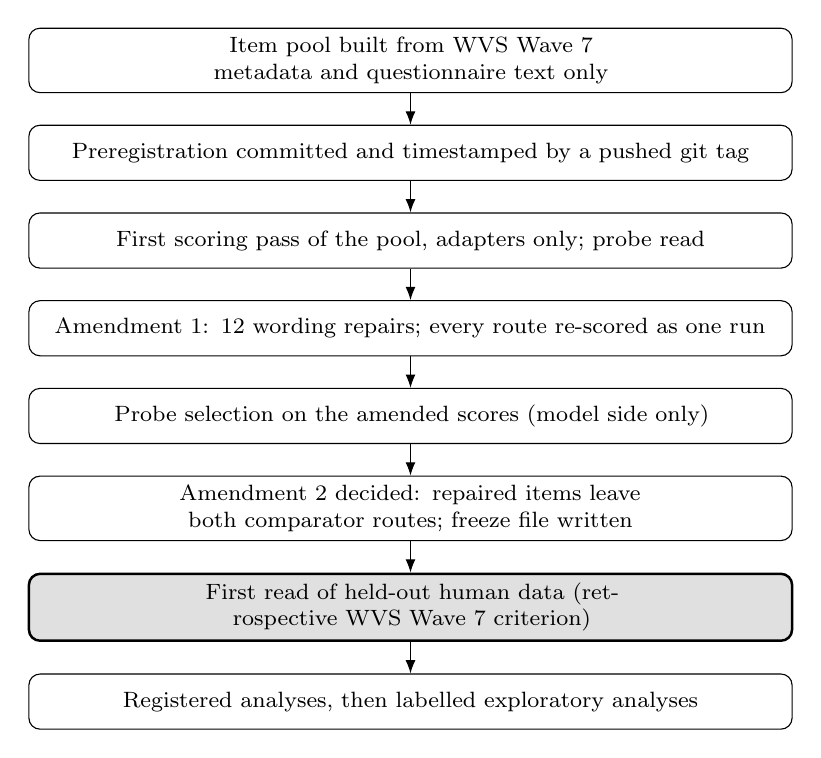
\begin{tikzpicture}[>=Latex,node distance=4mm,every node/.style={font=\footnotesize,align=center},
  wstep/.style={draw,rounded corners,text width=0.78\textwidth,minimum height=7mm},
  human/.style={wstep,fill=black!12,line width=0.9pt}]
\node[wstep] (pool) {Item pool built from WVS Wave~7 metadata and questionnaire text only};
\node[wstep,below=of pool] (tag) {Preregistration committed and timestamped by a pushed git tag};
\node[wstep,below=of tag] (s1) {First scoring pass of the pool, adapters only; probe read};
\node[wstep,below=of s1] (a1) {Amendment 1: \dc{12}{repaired_items} wording repairs; every route re-scored as one run};
\node[wstep,below=of a1] (sel) {Probe selection on the amended scores (model side only)};
\node[wstep,below=of sel] (a2) {Amendment 2 decided: repaired items leave both comparator routes; freeze file written};
\node[human,below=of a2] (join) {First read of held-out human data (retrospective WVS Wave~7 criterion)};
\node[wstep,below=of join] (exp) {Registered analyses, then labelled exploratory analyses};
\foreach \a/\b in {pool/tag,tag/s1,s1/a1,a1/sel,sel/a2,a2/join,join/exp} \draw[->] (\a)--(\b);
\end{tikzpicture}
\caption{Order of work for the held-out screen. Every step above the shaded box used model scores, metadata or questionnaire text only. The shaded box is the single read of held-out human data.}\label{fig:timeline}
\end{figure}

\subsection{The sign-profile factorial}\label{sec:design-factorial}

The second cohort covers all \dc{64}{cells} sign profiles, so the strict-battery composites form a full factorial in six binary factors. For each of the seven surfaces we fit the probe's regression (intercept, six sign bits coded $\pm\dc{0.5}{x_code}$, \dc{15}{interactions} two-way interactions, \dc{42}{error_df} error degrees of freedom). A main effect is the difference between the mean composites of profiles with the bit set and without it. Because the bits were assigned by design, this is a causal statement about the instrument, which acts on synthetic labels; it carries no implication about how preferences operate in people. Each bit has an own surface (patience owns two). The project's analysis plan set one acceptance check, separate from the held-out registration: at least \dc{4}{v5_required} of the six bits must move their own surface more than any other (V5), against a binomial reference with a one-in-seven chance of a hit. Exploratory scale-free views divide effects by each surface's standard deviation over the \dc{64}{cells} profiles, count the surfaces whose largest mover is their own bit, and report the first principal component's variance share and the mean absolute correlation between surfaces. The same analyses on the \dc{64}{cells} prompted profiles contrast two instruments that carry the same declared information.

\subsection{Retraining noise and the near-zero margin}\label{sec:design-noise}

One profile adapter was retrained under the same protocol without a fixed seed, which estimates a noise floor for the pipeline; we compare its scores with the original on both batteries. A predeclared sensitivity check also removes the training pairs of every dimension whose GPS coordinate lies within \dc{0.10}{near_zero_cut} of zero (the sign rule treats a coordinate just above zero like a large positive one) and refits two countries (Great Britain and Colombia), each beside a size-matched control. The contrast is refit minus control on the dimensions still in training, in profile standard deviations, read against the retrain's shift. The rule was to report the margin beside the main results and never to promote it.

\subsection{Descriptive follow-up analyses}\label{sec:design-desc}

Four further analyses were added after the registered results had been read. They are not preregistered, enter no registered family, and test no rule fixed in advance; we label their numbers D and read them as descriptions. Their human input is the WVS Wave~7 file used for the screen, so every comparison with respondents is retrospective. All use the strict battery and the \dc{42}{countries} countries.

\paragraph{Three columns.} For each of the seven surfaces we compute three Spearman correlations over countries: the adapter composite with the GPS coordinate of the surface's own dimension, the adapter composite with the Wave~7 composite of the same items, and that human composite with the GPS. The adapter columns use the first-cohort adapters (S1; the second cohort is in the supplement) with the profile-block bootstrap of Section~\ref{sec:design-bank}; the human--GPS interval resamples countries (seed \dc{20260905}{seed_country}). The human columns of risk taking cover one country fewer, because one country has no valid answer to the risk item.

\paragraph{Distance to the survey distributions.} For country $c$ and item $q$, the total variation distance between the model's option probabilities and the survey-weighted human answer shares is
\begin{equation*}
\mathrm{TVD}_{cq}=\tfrac{1}{2}\sum_j \bigl|\widehat{P}_c(j\mid x_q)-P^{H}_c(j\mid q)\bigr|,
\end{equation*}
where $j$ runs over the answer codes and $P^{H}_c$ is the share of valid human answers equal to $j$. The headline statistic is the mean over items within a country and then over countries, so that each country counts once. We score four cells on the same frozen stack: the base model, the first-cohort adapters, the country-named persona prompt on the base model (surface P), and the adapters with the persona prompt together (gates in the supplement). Contrasts are paired differences of country means. The interaction contrast is the adapters' effect with the persona prompt minus their effect without it, and zero means that the two add. Each contrast has a profile-block and a country interval (\dc{2,000}{boot_draws} draws each). The human answer shares enter the distances and are not reported.

\paragraph{Cross-talk decomposition.} Starting from the main effects of the second-cohort factorial (Section~\ref{sec:design-factorial}), we write the main-effects prediction of a surface at a country's sign profile as the sum over the six bits of each bit's main effect times its code, and split it into an own part (the surface's own bit) and a cross part (the other five). We correlate each part with the GPS coordinate of the surface's own dimension over the countries and report Var(cross)/Var(full). The decomposition is behavioral and uses model quantities and published GPS values only.

\paragraph{Held-out label recovery.} Training pairs were split once into a training part and a held-out part that the adapters never saw. For each first-cohort adapter we scored each held-out pair as the sequence log probability of the chosen and of the rejected completion, under the adapter and under the base model, in a further run on the same stack (gates in the supplement). Recovery, accuracy and base accuracy are defined in Section~\ref{sec:res-recovery}. This is a construction check on the synthetic labels and involves no human data.
\section{Results}\label{sec:results}

The results follow the chain. Sections~\ref{sec:res-bank} and \ref{sec:res-persona} ask what the instrument keeps of its anchor: the second-bank check, and a comparison with a country-named prompt and a sign prompt. Sections~\ref{sec:res-screen} to \ref{sec:res-readout} ask how the instrument relates to respondents on new items, in a preregistered screen whose criterion is retrospective. Sections~\ref{sec:res-factorial} and \ref{sec:res-noise} describe the instrument itself. Sections~\ref{sec:res-human} to \ref{sec:res-recovery} report descriptive follow-up analyses that were not preregistered (surface D): agreement with respondents, the distance to their answer distributions, the decomposition of the factorial's cross-talk, and held-out label recovery. Each number carries the label of its surface. Everything computed against the WVS Wave~7 file is retrospective, because that file existed before the instrument.

\subsection{Anchor to instrument: a second scenario bank}\label{sec:res-bank}

The first cohort encodes four of the six declared signs on the strict battery (S1). Over the \dc{42}{countries} countries, the adapter--GPS Spearman correlation is \cl{0.744}{B2_cohort1_trust_rho} \ci{0.500}{0.865}{B2_cohort1_trust_rho} for trust, \cl{0.435}{B2_cohort1_risktaking_rho} \ci{0.085}{0.686}{B2_cohort1_risktaking_rho} for risk taking, \cl{0.488}{B2_cohort1_posrecip_rho} \ci{0.120}{0.695}{B2_cohort1_posrecip_rho} for positive reciprocity, and \cl{0.406}{B2_cohort1_altruism_rho} \ci{0.020}{0.676}{B2_cohort1_altruism_rho} for altruism. These four are the imprint set that the held-out screen later uses.

When the scenario bank is replaced (S2, first column of Table~\ref{tab:checks}), trust keeps its agreement with the GPS, at \cl{0.803}{B2_bank2_trust_rho} \ci{0.615}{0.876}{B2_bank2_trust_rho}. The other three imprint dimensions keep positive point estimates, but their intervals now include zero, so \cl{1}{B2_n_imprint_kept} of the \cl{4}{B2_n_imprint_kept:n} imprint dimensions passes the second-bank check and \cl{3}{B2_n_imprint_dropped} do not. Under the rule fixed before the second cohort was trained, we write no sentence about risk taking, positive reciprocity or altruism carrying over to the second bank. The surfaces that were flat on the first bank stay flat on the second (online supplement).

The two banks agree closely when compared profile by profile. Over the \dc{26}{profiles_realized} shared profiles, the rank correlation between first-bank and second-bank composites is \cl{0.907}{B2_bank_to_bank_trust_spearman} \ci{0.774}{0.957}{B2_bank_to_bank_trust_spearman} for trust. Risk taking is the least stable surface, at \cl{0.544}{B2_bank_to_bank_risktaking_spearman} \ci{0.187}{0.772}{B2_bank_to_bank_risktaking_spearman}, which fits its loss on the second-bank check; the other surfaces agree more closely across banks (online supplement gives both the rank and the Pearson correlation for every surface). Bank-to-bank agreement measures how much the scenario text changes the instrument. It says nothing about people.

\subsection{Anchor to instrument: naming the country or stating the signs}\label{sec:res-persona}

The comparison a survey researcher would reach for first is a prompt that names the population. Scored on the same stack, the country-named persona route does not reproduce the GPS trust order (P): its correlation over the \dc{42}{countries} countries is \cl{0.028}{PX_persona_trust_rho} \ci{-0.339}{0.381}{PX_persona_trust_rho}. The planned contrast with the first cohort is \cl{0.716}{PX_D_cohort1_trust} \ci{0.191}{1.154}{PX_D_cohort1_trust}, so on trust the adapters track the benchmark's order more closely than the named-country prompt, and the reading is the same under a country bootstrap. The sign-profile prompt, which states the same six signs in words, tracks trust as closely as the adapters, at \cl{0.773}{PX_signprompt_trust_rho} \ci{0.584}{0.844}{PX_signprompt_trust_rho}. On trust, what separates the routes is whether the declared sign is supplied, whichever channel carries it. The contrast sets declared signs against a country name and says nothing about trained weights against prompting. On the other surfaces the persona route carries part of the patience ordering, positively on one item and negatively on the other, and its remaining intervals include zero (online supplement).

\subsection{Instrument to respondents: the retrospective screen}\label{sec:res-screen}

Retrospectively, the screen rejects its registered null. The probe selected \cl{56}{SCR_A_primary:n} of the \dc{223}{pool_items} pool items under the primary rule. Their mean signed agreement with the WVS Wave~7 country differences is $A=\cl{0.061}{SCR_A_primary}$, with a country-bootstrap interval of \ci{-0.007}{0.126}{SCR_A_primary}. Under the permutation null, which reassigns the same dimension and sign pairs to items drawn at random from the pool, the null distribution has mean \cl{0.012}{SCR_null_mean} and ninety-fifth percentile \cl{0.046}{SCR_null_q95}, and the one-sided $p$ is \cl{0.010}{SCR_p_perm}. Item--country cells that were never fielded enter as missing (online supplement).

By the registered reading, the signal is weak. Two WVS waves agree with each other on the selected items fielded in both waves with a mean Spearman correlation of \cl{0.746}{SCR_ceiling_mean} (median \cl{0.767}{SCR_ceiling_median}, \cl{34}{SCR_ceiling_mean:n} items). The screen's $A$ is \cl{8.1}{SCR_A_over_ceiling:pct}\% of that ceiling, well below the registered bar of one third, which would be \cl{0.249}{SCR_one_third_ceiling}. The bootstrap interval reaches zero while the permutation test rejects the null because the two answer different questions: whether the assignments beat random assignments of the same pairs to items from the same pool, and how much $A$ varies across samples of countries. The direction of the finding is clearer than its size.

The registered reliability checks point the same way. The secondary rule gives $A=\cl{0.070}{SCR_secondary_A}$ over \cl{185}{SCR_secondary_A:n} items with a one-sided permutation $p\cl{<0.001}{SCR_secondary_p_perm}$, and dropping one country at a time moves the primary $A$ only between \cl{0.051}{SCR_loco_min} and \cl{0.072}{SCR_loco_max}. An exploratory check against each wave's country means, on the items fielded in both waves, shows that the small signal does not depend on one wave (online supplement).

% Table 2: both checks per imprint dimension. Every number is a \cl / \ci macro tied to NUMBERS_TABLE.csv.
\begin{table}[htbp]
\centering
\caption{The second-bank check and the retrospective screen, by imprint dimension. The two checks are reported side by side and never averaged.}\label{tab:checks}
\small
\renewcommand{\arraystretch}{1.2}
\begin{tabularx}{\textwidth}{@{}>{\raggedright\arraybackslash}p{0.17\textwidth}>{\raggedright\arraybackslash}X>{\raggedright\arraybackslash}X>{\raggedright\arraybackslash}X>{\raggedright\arraybackslash}X@{}}
\toprule
 & S2: second bank & H: primary rule & H: primary rule, Bonferroni & H: secondary rule \\
Dimension & $\rho$ [\dc{95}{ci_level}\% interval] & $A_d$ [\dc{95}{ci_level}\% interval], items & $A_d$ [adjusted interval] & $A_d$ [\dc{95}{ci_level}\% interval], items \\
\midrule
Trust & \cl{0.803}{B2_bank2_trust_rho} \newline \ci{0.615}{0.876}{B2_bank2_trust_rho}
 & \cl{0.062}{PD_adapter_primary_trust_A} \newline \ci{-0.047}{0.173}{PD_adapter_primary_trust_A}, \cl{12}{PD_adapter_primary_trust_A:n}
 & \ci{-0.088}{0.199}{PD_adapter_primary_trust_A_bonf}
 & \cl{0.092}{PD_adapter_secondary_trust_A} \newline \ci{-0.019}{0.199}{PD_adapter_secondary_trust_A}, \cl{44}{PD_adapter_secondary_trust_A:n} \\
Risk taking & \cl{0.210}{B2_bank2_risktaking_rho} \newline \ci{-0.199}{0.584}{B2_bank2_risktaking_rho}
 & \cl{0.158}{PD_adapter_primary_risktaking_A} \newline \ci{0.015}{0.290}{PD_adapter_primary_risktaking_A}, \cl{13}{PD_adapter_primary_risktaking_A:n}
 & \ci{-0.026}{0.326}{PD_adapter_primary_risktaking_A_bonf}
 & \cl{0.143}{PD_adapter_secondary_risktaking_A} \newline \ci{0.045}{0.229}{PD_adapter_secondary_risktaking_A}, \cl{50}{PD_adapter_secondary_risktaking_A:n} \\
Positive reciprocity & \cl{0.366}{B2_bank2_posrecip_rho} \newline \ci{-0.068}{0.652}{B2_bank2_posrecip_rho}
 & \cl{-0.071}{PD_adapter_primary_posrecip_A} \newline \ci{-0.281}{0.154}{PD_adapter_primary_posrecip_A}, \cl{11}{PD_adapter_primary_posrecip_A:n}
 & \ci{-0.332}{0.205}{PD_adapter_primary_posrecip_A_bonf}
 & \cl{-0.049}{PD_adapter_secondary_posrecip_A} \newline \ci{-0.198}{0.117}{PD_adapter_secondary_posrecip_A}, \cl{22}{PD_adapter_secondary_posrecip_A:n} \\
Altruism & \cl{0.364}{B2_bank2_altruism_rho} \newline \ci{-0.057}{0.653}{B2_bank2_altruism_rho}
 & \cl{0.069}{PD_adapter_primary_altruism_A} \newline \ci{-0.036}{0.177}{PD_adapter_primary_altruism_A}, \cl{20}{PD_adapter_primary_altruism_A:n}
 & \ci{-0.058}{0.198}{PD_adapter_primary_altruism_A_bonf}
 & \cl{0.040}{PD_adapter_secondary_altruism_A} \newline \ci{-0.038}{0.117}{PD_adapter_secondary_altruism_A}, \cl{69}{PD_adapter_secondary_altruism_A:n} \\
\bottomrule
\end{tabularx}
\par\smallskip
\begin{minipage}{\textwidth}\footnotesize
\textit{Note:} S2 is the Spearman correlation between second-bank adapter composites and the GPS coordinate over \dc{42}{countries} countries, with a profile-block bootstrap (\dc{2,000}{boot_draws} draws, seed \dc{20261011}{seed_c3}); model side only. H is the retrospective screen against WVS Wave~7 country means: $A_d$ is the mean signed item agreement over the selected items the instrument assigned to the dimension, with the registered country bootstrap (\dc{2,000}{boot_draws} resamples, seed \dc{20261015}{seed_screen}). The registered intervals are unadjusted. The Bonferroni intervals over the \dc{4}{imprint_dims} imprint dimensions are exploratory and read off the same draws. The secondary rule is a registered reliability check. No dimension has an interval above zero on both S2 and H.
\end{minipage}
\end{table}


The per-dimension readings show where the signal sits (Table~\ref{tab:checks}). Under the primary rule, only the items assigned to risk taking have an interval above zero, $A_d=\cl{0.158}{PD_adapter_primary_risktaking_A}$ \ci{0.015}{0.290}{PD_adapter_primary_risktaking_A} on \cl{13}{PD_adapter_primary_risktaking_A:n} items, of which \cl{92.3}{PD_adapter_primary_risktaking_share_pos:pct}\% agree in sign. The intervals for trust and altruism include zero. The items assigned to positive reciprocity point the wrong way: their point estimate is negative, and only \cl{18.2}{PD_adapter_primary_posrecip_share_pos:pct}\% of the \cl{11}{PD_adapter_primary_posrecip_share_pos:n} items agree in sign. The secondary rule agrees on both points (online supplement).\footnote{The probe's per-dimension permutation $p$ values were not registered. For altruism under the primary rule they point the other way from the registered interval, so we report the registered intervals only.}

These per-dimension intervals are unadjusted for testing four dimensions. In the exploratory Bonferroni adjustment, the primary-rule interval for risk taking becomes \ci{-0.026}{0.326}{PD_adapter_primary_risktaking_A_bonf} and includes zero, so the one primary-rule dimension that excludes zero does not survive.

The two checks in Table~\ref{tab:checks} disagree by dimension. Trust is the dimension that survives the second bank, and its retrospective screen interval includes zero. Risk taking is the dimension whose screen interval excludes zero before adjustment, and it is one of the three that lose their interval on the second bank. No imprint dimension passes both checks, and the per-dimension cells are small.

\subsection{Instrument to respondents: questionnaire readers and the prompt route}\label{sec:res-comparators}

% Table 3: registered contrasts with the questionnaire comparators and with the prompt route (surface H, retrospective).
\begin{table}[htbp]
\centering
\caption{Retrospective screen: the adapters against two questionnaire readers and against prompting with the same signs.}\label{tab:comparators}
\small
\renewcommand{\arraystretch}{1.2}
\begin{tabularx}{\textwidth}{@{}>{\raggedright\arraybackslash}p{0.24\textwidth}>{\raggedright\arraybackslash}X>{\raggedright\arraybackslash}X>{\raggedright\arraybackslash}X@{}}
\toprule
 & Face-valid reader & Typed decision model, majority of \dc{5}{jev_runs} runs & Sign-profile prompt \\
\midrule
Items assigned by both routes & \cl{5}{CMP_face_valid_D_common:n} & \cl{9}{CMP_jev_D_common:n} & \cl{16}{SP_overlap_with_adapter} \\
Same dimension and sign on those items & \cl{1}{CMP_face_valid_common_same_dim_sign} & \cl{7}{CMP_jev_common_same_dim_sign} & \cl{6}{SP_overlap_same_dim_sign} \\
Adapter minus route, shared items & \cl{0.020}{CMP_face_valid_D_common} \newline \ci{-0.181}{0.215}{CMP_face_valid_D_common} & \cl{-0.002}{CMP_jev_D_common} \newline \ci{-0.064}{0.061}{CMP_jev_D_common} & \cl{0.004}{SP_D_common} \newline \ci{-0.065}{0.075}{SP_D_common} \\
Adapter minus route, own items & \cl{-0.034}{CMP_face_valid_D_own} \newline \ci{-0.242}{0.169}{CMP_face_valid_D_own} & \cl{-0.067}{CMP_jev_D_own} \newline \ci{-0.237}{0.103}{CMP_jev_D_own} & \cl{0.033}{SP_D_own} \newline \ci{-0.083}{0.143}{SP_D_own} \\
Route's own $A$ (items) & \cl{0.095}{CMP_face_valid_A_imprint} (\cl{25}{CMP_face_valid_A_imprint:n}) & \cl{0.128}{CMP_jev_A_imprint} (\cl{40}{CMP_jev_A_imprint:n}) & \cl{0.028}{SP_A_primary} (\cl{56}{SP_A_primary:n}) \\
\bottomrule
\end{tabularx}
\par\smallskip
\begin{minipage}{\textwidth}\footnotesize
\textit{Note:} Differences are adapter minus the named route, with \dc{95}{ci_level}\% intervals from the paired country bootstrap (\dc{2,000}{boot_draws} resamples). The registered primary contrast with each questionnaire reader is the one on shared items. The questionnaire readers' own items are restricted to the imprint set, with the \dc{12}{repaired_items} items repaired by Amendment~1 removed. The adapter's own $A$ is \cl{0.061}{SCR_A_primary} on \cl{56}{SCR_A_primary:n} items. Every interval in the table covers zero.
\end{minipage}
\end{table}


The registered contrasts do not distinguish the adapters from a careful reader of the questionnaire (Table~\ref{tab:comparators}). Every interval covers zero, which the preregistration reads as ``the adapters match a careful reader''. That reading rests on few items. The coverage-matched contrasts use the \cl{5}{CMP_face_valid_D_common:n} items that the adapters and the face-valid rule both assign and the \cl{9}{CMP_jev_D_common:n} items they share with the typed decision model, and the routes agree on dimension and sign for \cl{1}{CMP_face_valid_common_same_dim_sign} and \cl{7}{CMP_jev_common_same_dim_sign} of them. An interval that covers zero on so few items is consistent with a match and does not establish one. Both readers concentrate on trust, where their own-item $A$ exceeds the \cl{0.062}{PD_adapter_primary_trust_A} of the adapters' own trust items, but their per-dimension cells hold too few items to be informative.

Prompting the base model with the same six signs does not pass the registered null. The same probe applied to the \dc{64}{cells} prompted profiles gives $A=\cl{0.028}{SP_A_primary}$ \ci{-0.109}{0.158}{SP_A_primary} with a one-sided permutation $p$ of \cl{0.509}{SP_p_perm}, and it assigns its selected items to a single dimension, trust. The adapter route passes the null and the prompt route does not, but the direct difference between them is unresolved: adapter minus prompt is \cl{0.033}{SP_D_own} on each route's own items and \cl{0.004}{SP_D_common} on the \cl{16}{SP_overlap_with_adapter} items both select, and both intervals cover zero. The two routes agree on dimension and sign for \cl{6}{SP_overlap_same_dim_sign} of those shared items. The paper therefore cannot credit the trained weights over the prompt on the screen.

\subsection{Instrument to respondents: readout robustness}\label{sec:res-readout}

Item-level assignment is stable under option order and paraphrase, whereas membership in the particular selected set churns. The registered statistic, the number of selected items whose dimension and sign are unchanged, is \cl{39}{RO_heldout_reverse_ds_unchanged} of \cl{56}{RO_heldout_reverse_ds_unchanged:n} with reversed options, \cl{39}{RO_heldout_para_a_ds_unchanged} with the first paraphrase and \cl{30}{RO_heldout_para_b_ds_unchanged} with the second. No variant changes more than half, so the registered condition for wording dependence is not met, although the second paraphrase comes close. Membership is another matter: the primary rule is a top-quartile cut on $|t|$, small shifts reorder items near the cut, and only \cl{18}{RO_heldout_reverse_membership_agreement}, \cl{29}{RO_heldout_para_a_membership_agreement} and \cl{16}{RO_heldout_para_b_membership_agreement} of the \cl{56}{RO_heldout_para_b_membership_agreement:n} items are selected under both the original readout and the respective variant (online supplement). A researcher who reads the instrument should trust the dimension and direction it assigns to an item more than the list of items it ranks highest.

\subsection{Inside the instrument: the sign-profile factorial}\label{sec:res-factorial}

% Table 4: the sign-profile factorial on the strict battery (surface F, model side only).
\begin{table}[htbp]
\centering
\caption{Own effects of the six sign bits and summary of entanglement, by route. Strict battery, all \dc{64}{cells} sign profiles.}\label{tab:factorial}
\small
\renewcommand{\arraystretch}{1.15}
\begin{tabularx}{\textwidth}{@{}>{\raggedright\arraybackslash}X r r r r@{}}
\toprule
 & \multicolumn{2}{c}{Trained adapters} & \multicolumn{2}{c}{Sign-profile prompt} \\
\cmidrule(lr){2-3}\cmidrule(l){4-5}
Own effect on surface & Main effect & $t$ & Main effect & $t$ \\
\midrule
Trust & \cl{0.364}{FX_adapter64_trust_own_beta} & \cl{16.74}{FX_adapter64_trust_own_t} & \cl{1.780}{FX_signprompt64_trust_own_beta} & \cl{394.46}{FX_signprompt64_trust_own_t} \\
Negative reciprocity & \cl{0.625}{FX_adapter64_negrecip_own_beta} & \cl{11.64}{FX_adapter64_negrecip_own_t} & \cl{-0.023}{FX_signprompt64_negrecip_own_beta} & \cl{-1.80}{FX_signprompt64_negrecip_own_t} \\
Altruism & \cl{0.242}{FX_adapter64_altruism_own_beta} & \cl{6.32}{FX_adapter64_altruism_own_t} & \cl{0.364}{FX_signprompt64_altruism_own_beta} & \cl{11.99}{FX_signprompt64_altruism_own_t} \\
Patience (Q50) & \cl{0.133}{FX_adapter64_patience_Q50_own_beta} & \cl{6.12}{FX_adapter64_patience_Q50_own_t} & \cl{0.421}{FX_signprompt64_patience_Q50_own_beta} & \cl{17.63}{FX_signprompt64_patience_Q50_own_t} \\
Risk taking & \cl{0.140}{FX_adapter64_risktaking_own_beta} & \cl{4.14}{FX_adapter64_risktaking_own_t} & \cl{-0.457}{FX_signprompt64_risktaking_own_beta} & \cl{-22.31}{FX_signprompt64_risktaking_own_t} \\
Patience (Q43) & \cl{0.049}{FX_adapter64_patience_Q43_own_beta} & \cl{3.63}{FX_adapter64_patience_Q43_own_t} & \cl{-0.069}{FX_signprompt64_patience_Q43_own_beta} & \cl{-19.75}{FX_signprompt64_patience_Q43_own_t} \\
Positive reciprocity & \cl{0.124}{FX_adapter64_posrecip_own_beta} & \cl{3.02}{FX_adapter64_posrecip_own_t} & \cl{0.103}{FX_signprompt64_posrecip_own_beta} & \cl{5.66}{FX_signprompt64_posrecip_own_t} \\
\midrule
Summary of entanglement & \multicolumn{2}{r}{Trained adapters} & \multicolumn{2}{r}{Sign-profile prompt} \\
\midrule
Own effects against the intended direction & \multicolumn{2}{r}{\cl{0}{FX_adapter64_own_effects_wrong_signed} of \cl{7}{FX_adapter64_own_effects_wrong_signed:n}} & \multicolumn{2}{r}{\cl{3}{FX_signprompt64_own_effects_wrong_signed} of \cl{7}{FX_signprompt64_own_effects_wrong_signed:n}} \\
Bits dominant on their own surface (V5) & \multicolumn{2}{r}{\cl{2}{FX_adapter64_V5_hits} of \cl{6}{FX_adapter64_V5_hits:n}} & \multicolumn{2}{r}{\cl{2}{FX_signprompt64_V5_hits} of \cl{6}{FX_signprompt64_V5_hits:n}} \\
Same, on standardized effects & \multicolumn{2}{r}{\cl{2}{FX_adapter64_rowwise_standardized_hits} of \cl{6}{FX_adapter64_rowwise_standardized_hits:n}} & \multicolumn{2}{r}{\cl{1}{FX_signprompt64_rowwise_standardized_hits} of \cl{6}{FX_signprompt64_rowwise_standardized_hits:n}} \\
Surfaces whose largest mover is their own bit & \multicolumn{2}{r}{\cl{1}{FX_adapter64_columnwise_hits} of \cl{7}{FX_adapter64_columnwise_hits:n}} & \multicolumn{2}{r}{\cl{1}{FX_signprompt64_columnwise_hits} of \cl{7}{FX_signprompt64_columnwise_hits:n}} \\
Surfaces whose largest mover is the trust bit & \multicolumn{2}{r}{\cl{3}{FX_adapter64_surfaces_largest_mover_is_trust_bit} of \cl{7}{FX_adapter64_surfaces_largest_mover_is_trust_bit:n}} & \multicolumn{2}{r}{\cl{7}{FX_signprompt64_surfaces_largest_mover_is_trust_bit} of \cl{7}{FX_signprompt64_surfaces_largest_mover_is_trust_bit:n}} \\
Variance on the first principal component & \multicolumn{2}{r}{\cl{51.3}{FX_adapter64_pc1_share:pct}\%} & \multicolumn{2}{r}{\cl{83.5}{FX_signprompt64_pc1_share:pct}\%} \\
Mean absolute correlation between surfaces & \multicolumn{2}{r}{\cl{0.395}{FX_adapter64_mean_abs_inter_surface_r}} & \multicolumn{2}{r}{\cl{0.807}{FX_signprompt64_mean_abs_inter_surface_r}} \\
\bottomrule
\end{tabularx}
\par\smallskip
\begin{minipage}{\textwidth}\footnotesize
\textit{Note:} Main effects are differences in mean surface composite between profiles with the bit set and without it, from an OLS fit with the six bits and their \dc{15}{interactions} two-way interactions (\dc{42}{error_df} error degrees of freedom); composites are expected recoded responses averaged over the surface's items, so the units differ across surfaces. The manipulation is of synthetic training labels or prompted signs; the effects are changes in model response distributions. V5 was a planned acceptance check (at least \dc{4}{v5_required} of \dc{6}{sign_bits} bits); the other summary rows are exploratory.
\end{minipage}
\end{table}


On the trained route, every sign bit moves its own surface in the intended direction (Table~\ref{tab:factorial}). All seven own effects are positive, from \cl{0.364}{FX_adapter64_trust_own_beta} for trust ($t=\cl{16.74}{FX_adapter64_trust_own_t}$) to \cl{0.124}{FX_adapter64_posrecip_own_beta} for positive reciprocity ($t=\cl{3.02}{FX_adapter64_posrecip_own_t}$), and \cl{0}{FX_adapter64_own_effects_wrong_signed} of \cl{7}{FX_adapter64_own_effects_wrong_signed:n} point the wrong way.

The planned separability check fails. Only \cl{2}{FX_adapter64_V5_hits} of the \cl{6}{FX_adapter64_V5_hits:n} bits, those for altruism and negative reciprocity, move their own surface more than any other surface, where at least \dc{4}{v5_required} were required (binomial $p=\cl{0.207}{FX_adapter64_V5_p_binomial}$). The scale-free views agree: \cl{2}{FX_adapter64_rowwise_standardized_hits} of \cl{6}{FX_adapter64_rowwise_standardized_hits:n} on standardized effects, and \cl{1}{FX_adapter64_columnwise_hits} of \cl{7}{FX_adapter64_columnwise_hits:n} surfaces, trust, whose largest mover is its own bit. Each bit moves its own surface and also moves others, often by more: the risk-taking bit moves the altruism surface by \cl{0.983}{FX_adapter64_risktaking_bit_on_altruism}, against the altruism bit's own effect of \cl{0.242}{FX_adapter64_altruism_own_beta}, and the trust bit is the largest mover on \cl{3}{FX_adapter64_surfaces_largest_mover_is_trust_bit} of the \cl{7}{FX_adapter64_surfaces_largest_mover_is_trust_bit:n} surfaces. One common direction carries \cl{51.3}{FX_adapter64_pc1_share:pct}\% of the variance of the seven standardized surfaces, and the mean absolute correlation between surfaces is \cl{0.395}{FX_adapter64_mean_abs_inter_surface_r}. The sign bits are inputs that the instrument keeps distinct in direction and mixes in magnitude.

The prompted route fails the separability check by the same count, \cl{2}{FX_signprompt64_V5_hits} of \cl{6}{FX_signprompt64_V5_hits:n} (binomial $p=\cl{0.207}{FX_signprompt64_V5_p_binomial}$), so V5 does not separate the routes. The common direction and the sign of the own effects do. Under prompting, the first principal component carries \cl{83.5}{FX_signprompt64_pc1_share:pct}\% of the variance, the mean absolute correlation between surfaces is \cl{0.807}{FX_signprompt64_mean_abs_inter_surface_r}, and the trust bit is the largest mover on all \cl{7}{FX_signprompt64_surfaces_largest_mover_is_trust_bit} surfaces. Three prompted own effects point against the intended direction: risk taking at \cl{-0.457}{FX_signprompt64_risktaking_own_beta} ($t=\cl{-22.31}{FX_signprompt64_risktaking_own_t}$), patience Q43 at \cl{-0.069}{FX_signprompt64_patience_Q43_own_beta} ($t=\cl{-19.75}{FX_signprompt64_patience_Q43_own_t}$), and negative reciprocity at \cl{-0.023}{FX_signprompt64_negrecip_own_beta}, which at $t=\cl{-1.80}{FX_signprompt64_negrecip_own_t}$ is not distinguishable from zero. The contrast concerns entanglement and the direction of own effects. It is silent on screening accuracy, where the difference between routes is unresolved.

\subsection{Inside the instrument: retraining noise and the near-zero margin}\label{sec:res-noise}

The unseeded retrain of one profile reproduces the original adapter's readings closely. On the strict battery (\cl{140}{RP_strict_n_cells} scored cells), the largest single-cell difference in code probability is \cl{0.052}{RP_strict_max_abs_prob_diff} and the mean absolute difference is \cl{0.0060}{RP_strict_mean_abs_prob_diff}; the Pearson correlation of expected codes over the \cl{23}{RP_strict_pearson_expected_codes:n} items is \cl{0.9998}{RP_strict_pearson_expected_codes}. On the held-out pool (\cl{1{,}087}{RP_heldout_n_cells} cells), the corresponding values are \cl{0.092}{RP_heldout_max_abs_prob_diff}, \cl{0.0056}{RP_heldout_mean_abs_prob_diff} and \cl{0.9996}{RP_heldout_pearson_expected_codes} over \cl{223}{RP_heldout_pearson_expected_codes:n} items. Every strict-surface shift is at most \cl{0.112}{RP_max_abs_surface_diff_sd} of a standard deviation across profiles, with patience Q50 the largest. This bounds retraining noise for one unit; the variance of retraining across units was not measured.\footnote{Near-zero margin (surface N). The near-zero filter is not promoted under the predeclared rule. Colombia's positive reciprocity moved \cl{0.092}{NZ_COL_posrecip_refit_minus_control_sd:abs} profile standard deviations against its intended direction relative to its control, beyond the declared replicate floor of \cl{0.011}{NZ_COL_posrecip_noise_floor_sd}. A size-matched control, however, differs from the full-data baseline by up to \cl{1.222}{NZ_GBR_max_abs_control_minus_baseline_sd} standard deviations for Great Britain and \cl{1.499}{NZ_COL_max_abs_control_minus_baseline_sd} for Colombia, so the floor is too small to read small-data refits against. We claim no reversal. Two refits are a screen, with no interval and no claim across countries (online supplement).}

\subsection{Instrument to respondents: agreement with the human composite}\label{sec:res-human}

The next four subsections report descriptive follow-up analyses (surface D). They were added after the registered results had been read. None is preregistered, none enters a registered family, and none earns a claim. They set the instrument beside the respondents of the WVS Wave~7 file on the strict battery, and every statement is retrospective. For each surface, Table~\ref{tab:human} gives three Spearman correlations over the \dc{42}{countries} countries: adapter composite with GPS, adapter composite with the human composite of the same items, and the human composite with GPS.

On trust, the first-cohort adapters track the GPS, \cl{0.744}{C9_a_adapter_gps_trust_spearman_rho} \ci{0.500}{0.865}{C9_a_adapter_gps_trust_spearman_rho}, and do not reach the human composite, \cl{0.295}{C9_a_adapter_human_trust_spearman_rho} \ci{-0.044}{0.547}{C9_a_adapter_human_trust_spearman_rho}. All seven adapter--human intervals include zero, and the largest point estimate belongs to negative reciprocity, \cl{0.389}{C9_a_adapter_human_negrecip_spearman_rho} \ci{-0.008}{0.694}{C9_a_adapter_human_negrecip_spearman_rho}. The second-cohort adapters give the same picture on trust, with an adapter--human correlation of \cl{0.340}{C9_b_adapter_human_trust_spearman_rho} \ci{-0.025}{0.586}{C9_b_adapter_human_trust_spearman_rho}; positive reciprocity is the one second-cohort interval that excludes zero, and only just (online supplement).

The link between the GPS and the human composite is itself loose on these items. Its interval excludes zero on four of the seven surfaces (Table~\ref{tab:human}): positive for trust, \cl{0.351}{C9_a_human_gps_trust_spearman_rho} \ci{0.088}{0.564}{C9_a_human_gps_trust_spearman_rho}, and negative for patience Q43, \cl{-0.533}{C9_a_human_gps_patience_q43_spearman_rho} \ci{-0.741}{-0.266}{C9_a_human_gps_patience_q43_spearman_rho}. We read this column as a reference for scale and not as a ceiling, because it does not bound a scorer that is nonlinear or constant within sign profiles. Together, the three columns say that the adapters carry the GPS order on trust, that the GPS order is only loosely related to the human composite, and that the adapters' order of countries does not detectably agree with the human composite on any surface.

% Table: three-column agreement of the first-cohort adapters on the strict battery (surface D; descriptive,
% not preregistered). Every number is a \cl / \ci macro tied to NUMBERS_TABLE.csv.
\begin{table}[htbp]
\centering
\caption{Agreement with the GPS and with the WVS Wave~7 composite, first-cohort adapters, strict battery (surface D, descriptive and not preregistered; retrospective). Spearman correlation over countries, by surface.}\label{tab:human}
\footnotesize
\setlength{\tabcolsep}{4pt}
\renewcommand{\arraystretch}{1.15}
\begin{tabularx}{\textwidth}{@{}>{\raggedright\arraybackslash}X l l l@{}}
\toprule
Surface & Adapter--GPS & Adapter--human & Human--GPS \\
\midrule
Trust & \cl{0.744}{C9_a_adapter_gps_trust_spearman_rho} \ci{0.500}{0.865}{C9_a_adapter_gps_trust_spearman_rho} & \cl{0.295}{C9_a_adapter_human_trust_spearman_rho} \ci{-0.044}{0.547}{C9_a_adapter_human_trust_spearman_rho} & \cl{0.351}{C9_a_human_gps_trust_spearman_rho} \ci{0.088}{0.564}{C9_a_human_gps_trust_spearman_rho} \\
Risk taking & \cl{0.435}{C9_a_adapter_gps_risktaking_spearman_rho} \ci{0.085}{0.686}{C9_a_adapter_gps_risktaking_spearman_rho} & \cl{0.120}{C9_a_adapter_human_risktaking_spearman_rho} \ci{-0.260}{0.426}{C9_a_adapter_human_risktaking_spearman_rho} & \cl{-0.059}{C9_a_human_gps_risktaking_spearman_rho} \ci{-0.429}{0.312}{C9_a_human_gps_risktaking_spearman_rho} \\
Positive reciprocity & \cl{0.488}{C9_a_adapter_gps_posrecip_spearman_rho} \ci{0.120}{0.695}{C9_a_adapter_gps_posrecip_spearman_rho} & \cl{0.324}{C9_a_adapter_human_posrecip_spearman_rho} \ci{-0.074}{0.619}{C9_a_adapter_human_posrecip_spearman_rho} & \cl{0.054}{C9_a_human_gps_posrecip_spearman_rho} \ci{-0.269}{0.386}{C9_a_human_gps_posrecip_spearman_rho} \\
Altruism & \cl{0.406}{C9_a_adapter_gps_altruism_spearman_rho} \ci{0.020}{0.676}{C9_a_adapter_gps_altruism_spearman_rho} & \cl{0.128}{C9_a_adapter_human_altruism_spearman_rho} \ci{-0.170}{0.369}{C9_a_adapter_human_altruism_spearman_rho} & \cl{0.031}{C9_a_human_gps_altruism_spearman_rho} \ci{-0.306}{0.350}{C9_a_human_gps_altruism_spearman_rho} \\
Negative reciprocity & \cl{-0.028}{C9_a_adapter_gps_negrecip_spearman_rho} \ci{-0.418}{0.406}{C9_a_adapter_gps_negrecip_spearman_rho} & \cl{0.389}{C9_a_adapter_human_negrecip_spearman_rho} \ci{-0.008}{0.694}{C9_a_adapter_human_negrecip_spearman_rho} & \cl{0.416}{C9_a_human_gps_negrecip_spearman_rho} \ci{0.173}{0.586}{C9_a_human_gps_negrecip_spearman_rho} \\
Patience (Q43) & \cl{-0.019}{C9_a_adapter_gps_patience_q43_spearman_rho} \ci{-0.414}{0.452}{C9_a_adapter_gps_patience_q43_spearman_rho} & \cl{0.192}{C9_a_adapter_human_patience_q43_spearman_rho} \ci{-0.169}{0.464}{C9_a_adapter_human_patience_q43_spearman_rho} & \cl{-0.533}{C9_a_human_gps_patience_q43_spearman_rho} \ci{-0.741}{-0.266}{C9_a_human_gps_patience_q43_spearman_rho} \\
Patience (Q50) & \cl{0.177}{C9_a_adapter_gps_patience_q50_spearman_rho} \ci{-0.313}{0.580}{C9_a_adapter_gps_patience_q50_spearman_rho} & \cl{0.003}{C9_a_adapter_human_patience_q50_spearman_rho} \ci{-0.291}{0.316}{C9_a_adapter_human_patience_q50_spearman_rho} & \cl{0.388}{C9_a_human_gps_patience_q50_spearman_rho} \ci{0.095}{0.628}{C9_a_human_gps_patience_q50_spearman_rho} \\
\bottomrule
\end{tabularx}
\par\smallskip
\begin{minipage}{\textwidth}\footnotesize
\textit{Note:} Each cell is the Spearman correlation with a \dc{95}{ci_level}\% interval. Over \dc{42}{countries} countries, except the two human columns of risk taking, which cover \cl{41}{C9_a_adapter_human_risktaking_spearman_rho:n} countries because one country has no valid answer to the risk item (Q178). Adapter intervals resample the \dc{26}{profiles_realized} sign profiles (\dc{2,000}{boot_draws} draws, seed \dc{20261011}{seed_c3}); the human--GPS interval resamples countries (seed \dc{20260905}{seed_country}). The human composite is the Wave~7 item-mean composite of the same strict-battery items. The adapter--GPS column repeats the S1 values of Section~\ref{sec:res-bank}.
\end{minipage}
\end{table}


\subsection{Instrument to respondents: distance to the survey distributions}\label{sec:res-tvd}

The correlations above concern the order of countries. A different question is how far the instrument's answer distribution lies from the survey's. For each country--item cell we take the total variation distance between the model's probabilities over the answer codes and the survey-weighted shares of valid human answers, and report its country-equal mean; lower is closer (Section~\ref{sec:design-desc}). Four cells are compared: the base model, the first-cohort country adapters, the country-named persona prompt, and the adapters and the persona prompt together.

The base model's mean distance is \cl{0.470}{C9_TVD_base_mean_tvd_country_equal}. The adapters sit farther from the survey, at \cl{0.515}{C9_TVD_adapter_mean_tvd_country_equal}, and the persona prompt sits closer, at \cl{0.365}{C9_TVD_persona_mean_tvd_country_equal}. Relative to the base model, the adapters are farther by \cl{0.045}{C9_TVD_adapter_minus_base_profile_block} \ci{0.006}{0.093}{C9_TVD_adapter_minus_base_profile_block} under profile blocks, and the persona prompt is closer by \cl{-0.105}{C9_TVD_persona_minus_base_profile_block} \ci{-0.122}{-0.086}{C9_TVD_persona_minus_base_profile_block}; country resampling gives the same readings (online supplement). By dimension, the adapters are farther than the base model on four of the six dimensions and slightly closer on the other two (point estimates; online supplement). With both interventions the distance is \cl{0.420}{C9_TVD_adapter_persona_mean_tvd_country_equal}. The interaction contrast, the adapters' effect with the persona prompt minus their effect without it, is \cl{0.009}{C9_TVD_interaction_profile_block} \ci{-0.003}{0.022}{C9_TVD_interaction_profile_block} under profile blocks, which includes zero, so the data show no detectable departure from additivity; descriptively, the adapters' step away from the survey and the persona prompt's step toward it are consistent with adding.

The ordering of the cells by distance does not follow their ordering by trust agreement with the GPS. The persona prompt has the lowest distance and no trust order (Section~\ref{sec:res-persona}). The adapters have the highest distance and keep the trust order, and adding the persona prompt to the adapters keeps the trust order while the distance falls. The two measures ask different questions, and neither says why the adapters' distributions lie where they do. The instrument carries no information about magnitudes (Section~\ref{sec:discussion}), so a distance to survey distributions is not a quantity it was built to reduce.

\subsection{Inside the instrument: why trust is spared}\label{sec:res-w1}

The factorial shows that each bit moves its own surface in the intended direction and also moves other surfaces (Section~\ref{sec:res-factorial}). To ask why the adapters keep the GPS order of countries on trust and lose it on most other surfaces, we split the main effects of the second-cohort adapters into the effect of each surface's own bit and the summed effect of the other five bits, evaluate each part at the sign profile of each of the \dc{42}{countries} countries, and correlate it with the GPS coordinate of the surface's own dimension (online supplement gives every surface). This is a behavioral decomposition of the adapters' main effects and says nothing about mechanism inside the network.

The own-bit part orders the countries like the GPS on all seven surfaces, with correlations from \cl{0.817}{C9_W1_patience_Q43_spearman_own_vs_gps} to \cl{0.866}{C9_W1_posrecip_spearman_own_vs_gps}. This is mechanical. For a positive own effect, as all seven are, the own part is proportional to the sign of the GPS coordinate, so it restates the correlation between the signs and the GPS and is not a separate test of learning. The full prediction, which adds the cross bits, keeps the GPS order on trust, \cl{0.834}{C9_W1_trust_spearman_full_vs_gps}, and loses most of it elsewhere, with correlations from \cl{-0.020}{C9_W1_patience_Q43_spearman_full_vs_gps} for patience Q43 to \cl{0.422}{C9_W1_altruism_spearman_full_vs_gps} for altruism.

The cross part carries little of the variation of the full prediction on trust and most of it elsewhere. Var(cross)/Var(full) is \cl{0.147}{C9_W1_trust_cross_var_share} on trust and runs from \cl{0.830}{C9_W1_negrecip_cross_var_share} to \cl{1.049}{C9_W1_patience_Q43_cross_var_share} on the other six. This is a ratio of variances and not a percentage of variance explained; it exceeds one on patience Q43 because the own and cross parts covary negatively. Interactions are needed on four surfaces, and they do not restore the GPS order (online supplement gives the covariance shares and the two-way correlations). The rank correlation across the seven surfaces between Var(cross)/Var(full) and the adapters' failure to order countries like the GPS rests on one surface, trust, set against six, so it is not a graded relation and we claim no dose--response (values in the online supplement). No bank label depends on a second dimension: in both banks all \cl{27{,}636}{C9_W1_bank1_label_rows_checked} country-pair training rows follow the sign of the pair's own dimension, with \cl{0}{C9_W1_bank1_label_mismatches} mismatches in the first bank and \cl{0}{C9_W1_bank2_label_mismatches} in the second, so the labels do not carry the cross-talk. We do not claim a cause of the loss on every surface. Component-level analysis, and interventions for any causal statement, have not been done.

\subsection{Anchor to instrument: held-out label recovery}\label{sec:res-recovery}

Every training pair of a country carries a label: the completion that goes with the sign of the country's GPS coordinate on the pair's own dimension is the chosen one. This construction check asks whether that installation carries over to pairs the adapters never saw. For each of the \dc{42}{countries} first-cohort adapters, the margin is the difference between the log probability of the chosen and of the rejected completion. Recovery is the share of held-out pairs on which the adapter's margin exceeds the base model's, accuracy is the share on which the adapter prefers its own chosen completion outright, and base accuracy is the same share for the base model. We report country-equal means with a profile-block bootstrap.

Recovery is \cl{0.940}{C9_label_recovery_recovery_profile_block} \ci{0.926}{0.952}{C9_label_recovery_recovery_profile_block} and accuracy is \cl{0.816}{C9_label_recovery_accuracy_profile_block} \ci{0.771}{0.856}{C9_label_recovery_accuracy_profile_block}. The base model's accuracy is \cl{0.489}{C9_label_recovery_base_accuracy_profile_block} \ci{0.471}{0.506}{C9_label_recovery_base_accuracy_profile_block}, an interval that includes one half, so the base model shows no detectable preference for the chosen completions before training. The mean margin shift is \cl{40.3}{C9_label_recovery_mean_margin_shift_profile_block} \ci{28.2}{54.1}{C9_label_recovery_mean_margin_shift_profile_block} nats. These checks show that training installed each country's synthetic labels on scenarios the adapter never saw. They say nothing about whether the labels order countries like the GPS and nothing about the respondents, and the distance results above show that the same adapters lie farther from the survey's answer distributions than the base model does.

\section{Discussion}\label{sec:discussion}

We set out to evaluate the sign compiler as a scoring instrument for new item text, and the evaluation returns a specific profile of what holds, what fails, and what remains untested. We take the three contributions in turn and then state the limits that apply to all of them.

\paragraph{The instrument.} Trained at full scale, the instrument encodes the direction of its declared signs: on the trained route, every sign bit moves its own surface the intended way, although only some of those surfaces agree with the GPS across countries (Section~\ref{sec:res-bank}). The magnitude of the encoding is fragile for most dimensions. Only trust keeps its agreement with the GPS when the scenario bank is replaced, and the bank-to-bank comparison locates risk taking as the dimension that the scenario text moves most (Section~\ref{sec:res-bank}). A researcher can therefore treat the instrument's trust surface as a property of the construction that survives a change of generator, and should treat the other surfaces as properties of a particular bank until a further bank says otherwise. Naming the country does not recover the trust order that the declared signs carry, whether the signs are trained into the adapters or stated in the prompt (Section~\ref{sec:res-persona}). This is a statement about the instrument and its anchor. It is silent on whether the WVS items measure the GPS constructs in people.

\paragraph{The retrospective screen.} The screen asked whether a probe that reads only the instrument picks items whose human country differences run in the assigned direction, and the registered answer is yes, weakly. The signal is a small fraction of what two human waves achieve on the same items, its bootstrap interval reaches zero, and it is concentrated in one dimension. That dimension, risk taking, is the one the second bank does not support, and its interval does not survive an exploratory adjustment for the four dimensions tested. Trust, the dimension that does survive the second bank, does not stand apart from zero in the screen. The items assigned to positive reciprocity point the wrong way. That disagreement could arise from the instrument, from the mapping between WVS items and the GPS construct, or from limited coherence between the two surveys for this dimension, and the design cannot separate these explanations. Read as cross-survey evidence, it marks positive reciprocity as the dimension on which the instrument's readings and the human survey part ways. On the items that the adapters share with two readers of the questionnaire, the registered contrasts cannot tell the adapters apart from those readers. The readers work mostly on trust and the overlap is small, so this comparison leaves open whether the adapters add anything a careful reader would miss on the dimensions the readers do not cover.

\paragraph{The diagnostic.} The factorial shows that the declared dimensions are entangled inside the instrument. Each bit moves its own surface the intended way, but the bits also move one another's surfaces, and a single common direction carries about half of the variance across surfaces. The planned separability check fails on both routes. Prompting with the same signs is more entangled still: one common direction dominates, the trust sign moves every surface, and three own effects point the wrong way. The same pattern appears on the held-out items, where the prompted probe assigned its selected items to trust alone and did not pass the null. Training on sign-labeled pairs is thus the route that keeps the direction of each declared input. It does not deliver separate dimensions. Because the two routes carry the same declared information, the contrast describes two instruments, and it makes no claim about which training recipe is best or about screening accuracy, where the difference between routes is unresolved.

\paragraph{Fidelity to labels and agreement with respondents.} The descriptive follow-up analyses (Sections~\ref{sec:res-human} to \ref{sec:res-recovery}) separate three parts of the construction that are easy to run together: the instrument, which turns declared signs into training labels; the anchor, which supplies the signs; and the model, which carries them. Fidelity to the labels is high. On training scenarios they never saw, the adapters' margins exceed the base model's on \cl{0.940}{C9_label_recovery_recovery_profile_block} of held-out pairs, and the adapters prefer their own chosen completion on \cl{0.816}{C9_label_recovery_accuracy_profile_block} of them, against \cl{0.489}{C9_label_recovery_base_accuracy_profile_block} for the base model. Agreement with respondents is a different fact. The same adapters sit farther from the survey's answer distributions than the base model, by \cl{0.045}{C9_TVD_adapter_minus_base_profile_block} \ci{0.006}{0.093}{C9_TVD_adapter_minus_base_profile_block} in total variation distance, whereas a country-named prompt, which involves no training, sits closer, by \cl{-0.105}{C9_TVD_persona_minus_base_profile_block} \ci{-0.122}{-0.086}{C9_TVD_persona_minus_base_profile_block}. The adapters' order of countries agrees with the GPS on trust and does not detectably agree with the human composite on any of seven surfaces. A model can therefore carry its declared inputs faithfully and still lie farther from respondents than a prompt that was never trained on those labels, and a construction check cannot stand in for a check against people. We read this as a point about how such an instrument should be evaluated, with the instrument, the anchor and the model each needing its own check, and not as a result about any one of them. The evidence is descriptive, it was not preregistered, it rests on one anchor and one human source, and it earns no claim. We do not test why the distributions move apart. The sign labels carry no information about magnitudes, the readout is a scoring convention, and the base model is shared, and the design cannot separate these.

\paragraph{Limits.} Five limits apply to every result above. First, the human criterion is retrospective. The WVS Wave~7 file existed before the probe, the pool and the adapters, and it is the only human source. Registration and the freeze guard protect against tuning the probe to the criterion, but they cannot make the criterion independent of the survey program from which the item pool was drawn. Pre-piloting, in the sense that screening with the instrument would change which items a researcher fields relative to a human-only rule declared in advance, is a prospective use that this paper does not test. Second, the instrument is built from signs. It carries no information about magnitudes, and it cannot represent differences among countries that share a sign profile or among people within a country. Its readings are group-level, and country-level agreement does not establish individual-level validity or measurement invariance \citep{davidov2014,bratt2025}. Third, every adapter shares one base model, one training recipe and one readout convention, and the readout's code probabilities are a scoring convention whose dispersion need not match human response distributions. Fourth, the per-dimension cells are small and the selected set churns under readout variants, so the instrument's item-level assignments are more stable than any particular list of selected items. Fifth, the noise checks are narrow: one unseeded retrain bounds retraining noise for one unit, and two near-zero refits are a screen with no claim across countries.

\paragraph{Intended use.} Within those limits, the instrument has a modest and inspectable use. A survey designer can read the dimension and direction it assigns to candidate items as one input beside expert review and human pretesting, keeping in view that no dimension passed both checks. Its value lies in what it makes explicit: the declared moments, the sign rule, and the absence of any group name at evaluation are all on the record, so a reader can see what information the instrument was given and check where its readings depart from people. It complements fielding and pretesting, and the evidence here gives no reason to use it in their place. In the terms of \citet{broska2025}, its readings are potentially informative observations that still require a human criterion.

\section{Conclusion}\label{sec:conclusion}

Synthetic cultural agents compile declared aggregate preference signs into choice policies that can be read on any survey item without naming a group. We evaluated them along the chain from anchor to instrument to respondents, and the evaluation says where they hold and where they fail.

Between anchor and instrument they hold in a limited sense. Training installs the synthetic labels on pairs the adapters never saw, and on trust the adapters keep the anchor's order of countries across a change of scenario bank. A prompt that names the country does not keep that order, and a prompt that states the same signs does, so the declared signs carry the trust order and the evidence cannot credit the trained weights over the prompt. The adapters do not keep the declared dimensions separate. Between instrument and respondents the evidence is weak. A preregistered screen of held-out items, read against a retrospective human criterion, gives a small signal that the registered comparisons do not separate from careful readers of the questionnaire. No dimension passes both the second-bank check and the screen, and the adapters' order of countries does not detectably agree with the respondents' composite. Keeping the anchor's order of countries and approaching respondents' answer distributions are different questions. On a descriptive reading that was not preregistered, the adapters keep the first and lie farther from the survey's answer distributions than the base model, whereas a country-named prompt lies closer with no trust order.

A researcher may use the instrument now as an inspectable, group-level reading of candidate items beside human pretesting, for which it is a complement and no replacement. The test that would license more is prospective: probe-selected items fielded to people after the selection and a human-only comparison rule have both been declared, so that the instrument's selections can be compared with what a researcher would otherwise have fielded. Until that test is run, pre-piloting remains untested.

% Backmatter in SMR order (venue card): preregistration; code, materials and data availability; institutional
% review; conflicting interests; funding; generative AI. Acknowledgements are on title_page.tex (anonymized review).
\section*{Preregistration Statement}

The held-out screen (Sections~\ref{sec:design-screen} and \ref{sec:res-screen}) was preregistered. The registration document was committed to the project repository and timestamped by the git tag \texttt{prereg-heldout-2026-10-14}, pushed before any held-out item was scored by an adapter. Amendment~1 (repair of \dc{12}{repaired_items} items whose standalone wording could not be answered) was made after the first model-side probe pass had been computed and read, and before any human value was read. The freeze file was committed, and Amendment~2 (removal of those items from both comparator routes) was decided, before the single read of held-out human data; the text of Amendment~2 was written afterwards and records that earlier decision. The criterion data, WVS Wave~7, are public and existed before the study, so the registration fixes the analysis before the authors read the human values and the criterion remains retrospective. All registered analyses of the screen are reported in Section~\ref{sec:res-screen} and Tables~\ref{tab:checks} and \ref{tab:comparators}, except two descriptives (item-level agreement after dropping items with small $|a_i|$, and the face-valid reader's statistic on all of its items including negative reciprocity), which are reported in the online supplement. % TODO(T10 follow-up): these two descriptives are not yet rows of NUMBERS_TABLE.csv; the supplement card must add them.
The Bonferroni intervals, the wave-specific screen statistics, the scale-free factorial views and the factorial route contrast are exploratory. The factorial's separability check (V5) was fixed in the project's analysis plan, separately from the registration. The second-bank decision rule was fixed before the second cohort was trained and was not part of the registration. An anonymized copy of the registration is provided with the submission. % TODO(Augusto): register the tagged document at an institutional registry (e.g., OSF). The registry copy will be dated after data access, and this statement must say so.

\section*{Code, Materials, and Data Availability}

Analysis code, the item pool and its overrides, the frozen selection, the comparator files, all model scores, and the scripts that build every number in this article from those scores are available for review at an anonymized link. % TODO(Augusto): anonymized mirror for review (e.g., anonymous.4open.science of the repository).
Model adapters and score archives are released at acceptance. The frozen inputs are identified by SHA-256 hashes: the amended item pool \clh{19241f6f103c51d6}{HASH_pool_worktree}\ldots{} as written to disk, whose line-ending-normalized form in the repository is \clh{a1dbceea1a33da05}{HASH_pool_git_blob_lf}\ldots{}; the overrides file \clh{0f5cd2bbd88ef6ea}{HASH_overrides}\ldots{}; and the frozen selection \clh{782b7d2123f9758e}{HASH_selection_amended_20261016}\ldots{}. The pool is regenerated byte for byte from the overrides file by the pool-building script; full hashes and the line-ending convention are in the online supplement. WVS and GPS data are available from their providers \citep{wvs2022,wvsts2022,falk2018} and are not redistributed; no respondent-level data or country-level human means are included in the replication materials.

\section*{Institutional Review}

This study analyzes publicly available, de-identified secondary survey data and involves no interaction with human participants. % TODO(Augusto): confirm the institutional review determination for secondary public data.

\section*{Declaration of Conflicting Interests}

The authors declared no potential conflicts of interest with respect to the research, authorship, and/or publication of this article. % TODO(Augusto): confirm for this paper (the confirmation on record covers the earlier preprint), including any relationship with the provider of the typed decision model used as a comparator.

\section*{Funding}

The authors received no financial support for the research, authorship, and/or publication of this article. % TODO(Augusto): confirm for this paper, including compute credits.

\section*{Declaration of Generative AI Use}

Large language models are the object of study in this article. In addition, an AI coding and writing assistant was used under the authors' direction to write analysis code and to draft and edit manuscript text; the authors reviewed all code, numbers and text and take responsibility for them. % TODO(Augusto): confirm wording and name the tools as SMR requires.

\singlespacing
\bibliographystyle{chicago}
\bibliography{references}
\end{document}
